\section{Durchführung}
\label{sec:Durchführung}

Der Versuchsaufbau ist in der folgenden Abbildung dargestellt
\begin{figure}
    \centering
    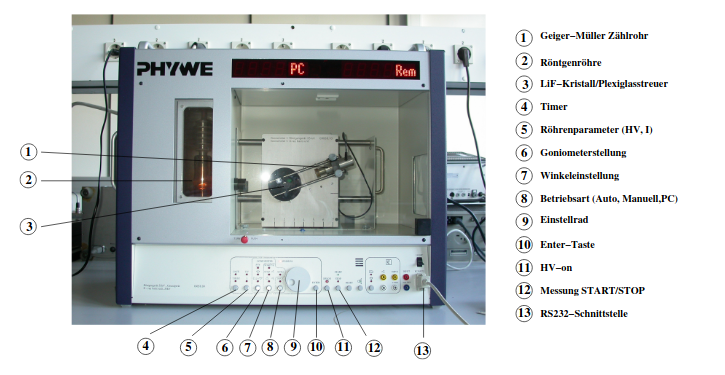
\includegraphics{Röntgenröhre.png}
    \caption{Experimenteller Versuchsaufbau \cite{anleitung}}
    \label{fig:hex}
  \end{figure}
Im Wesentlichen besteht er aus einer Röntgenröhre, einem LiF-Kristall und einem 
Geiger-Müller-Zählrohr. 
\\
\\
Zunächst wird zur Überprüfung der Braggbedingung der LiF-Kristall auf den festen Winkel 
$\theta = 14°$ eingestellt und der Winkel des Geiger-Müller-Zählrohrs um jeweils 
$\Delta \theta_{GM}$ im Winkelbereich zwischen 26° und 30° variiert.\\
Im nächsten Schritt wird nun das Emissionsspektrum in Schritten von $\Delta \theta = 0.1°$
mit einer Integrationszeit von $\Delta =10\ s$ gemessen.\\
Im Anschluss werden verschiedene Absorber - Zink, Gallium, Brom, Rubidium, Strontium und 
Zirkonium - vor dem Geiger-Müller-Zählrohr installiert und die 
Absorptionsspektren mit einer Genauigkeit von $0,1°$ und einer Integrationszeit 
von $\Delta t = 20 \ s$ aufgenommen.\\
Für Zink wurde der Winkelbereich von 18° bis 19,5° abgetastet.\\
Für Gallium wurde der Winkelbereich von 17° bis 19° abgetastet.\\
Für Brom wurde der Winkelbereich von 12,8° bis 14,2° abgetastet.\\
Für Rubidium wurde der Winkelbereich von 11,2° bis 12,5° abgetastet.\\
Für Strontium wurde der Winkelbereich von 10,5° bis 12° abgetastet.\\
Für Zirkonium wurde der Winkelbereich von 9,5° bis 11° abgetastet.\\